\chapter{Il pendolo di Kapitza}

In questa lezione studieremo un sistema meccanico derivato dal pendolo semplice detto pendolo di Kapitza. Il pendolo in questione è un pendolo semplice con cerniera superiore mobile e fatta oscillare ad una frequenza elevata con piccole oscillazioni. Sia $y_0(t)$ la posizione della cerniera.

\begin{center}
\begin{tikzpicture}[scale=1.2,>=Latex]
    \coordinate (O) at (0,0);
    \coordinate (M) at (1.8,-2.4);

    \draw[fill=white,line width=0.8pt] (O) circle (0.14);
    \node[left=4pt] at (O) {$O$};

    \draw[->,line width=0.9pt] (0,0.55) -- (0,0.15);
    \draw[->,line width=0.9pt] (0,-0.15) -- (0,-0.55);

    \draw[line width=0.9pt] (O) -- (M);
    \node[right] at (0.8,-1.0) {$\ell$};

    \fill (M) circle (0.14);
\end{tikzpicture}
\end{center}

Per modellizzare le piccole oscillazioni ad alta frequenza usiamo
\[
y_0(t)=a\cos(\omega t)
\qquad
a\ll \ell
\qquad
\omega \gg \sqrt{\frac{g}{\ell}}=\omega_0
\]

Dove $\ell$ e $\omega_0$ sono lunghezza e pulsazione del pendolo semplice.

Per scrivere le equazioni del moto di questo pendolo ci mettiamo nel sistema di riferimento (non inerziale) della cerniera. Devo aggiungere nel bilancio delle forze la forza apparente dovuta al moto della cerniera.

\[
y_0(t)=a\cos(\omega t)
\qquad \Rightarrow \qquad
\dot{y}_0(t)=-a\omega\sin(\omega t)
\qquad \Rightarrow \qquad
\ddot{y}_0(t)=-a\omega^2\cos(\omega t)
\]

Notiamo che nel nuovo sistema di riferimento non inerziale il polo appare di nuovo incernierato

\begin{center}
\begin{tikzpicture}[scale=1.25,>=Latex]
    \definecolor{mygreen}{RGB}{130,180,60}
    \definecolor{myred}{RGB}{210,40,30}

    % assi
    \draw[mygreen,->,line width=0.9pt] (-1.6,0.8) -- (-0.55,0.8);
    \node[mygreen,above] at (-1.0,0.8) {$\hat{\imath}$};

    \draw[mygreen,->,line width=0.9pt] (-1.6,0.8) -- (-1.6,1.8);
    \node[mygreen,left] at (-1.6,1.4) {$\hat{k}$};

    \draw[mygreen,line width=0.8pt] (-2.0,0.45) circle (0.18);
    \draw[mygreen,line width=0.8pt] (-2.1,0.35) -- (-1.9,0.55);
    \draw[mygreen,line width=0.8pt] (-2.1,0.55) -- (-1.9,0.35);
    \node[mygreen,left] at (-2.1,0.45) {$\hat{\jmath}$};

    % pendolo
    \coordinate (P) at (0,1.2);
    \coordinate (V) at (0,-0.2);
    \coordinate (M) at ($(P)+(-65:1.55)$);

    \draw[dashed,line width=0.8pt] (P) -- (V);
    \draw[line width=0.9pt] (P) -- (M);

    \draw[line width=0.8pt] (P) circle (0.12);
    \draw[line width=0.8pt] ($(P)+(-0.08,-0.08)$) -- ($(P)+(0.08,0.08)$);
    \draw[line width=0.8pt] ($(P)+(-0.08,0.08)$) -- ($(P)+(0.08,-0.08)$);

    \fill (M) circle (0.14);

    % angolo theta senza libreria angles
    \draw[->,line width=0.8pt]
        ($(P)+(0,-0.45)$) arc[start angle=-90,end angle=-65,radius=0.45];

    \node at ($(P)+(-77:0.65)$) {$\theta$};

    % forze
    \draw[myred,->,line width=0.9pt] (M) -- ++(0,1.05);
    \node[myred,right] at ($(M)+(0,0.55)$) {$ma\omega^2\cos(\omega t)$};

    \draw[mygreen,->,line width=0.9pt] (M) -- ++(0,-1.0);
    \node[mygreen,right] at ($(M)+(0,-0.55)$) {$mg$};
\end{tikzpicture}
\end{center}

Scrivo la seconda equazione cardinale
\[
\frac{d}{dt}\left(\underline{\ell}\wedge m\ell\dot{\theta}\,\hat{t}\right)
=
\underline{\ell}\wedge -mg\hat{k}
+
\underline{\ell}\wedge ma\omega^2\cos(\omega t)\hat{k}
\]

\[
\frac{d}{dt}\left(-\ell^2m\dot{\theta}\right)
=
+mg\ell\sin\theta
-\ell ma\omega^2\cos(\omega t)\sin\theta
\Longleftrightarrow
\ddot{\theta}
=
-\frac{g}{\ell}\sin\theta
+
\frac{m\ell a\omega^2}{m\ell^2}\cos(\omega t)\sin\theta
\]

\[
\Longleftrightarrow
\ddot{\theta}
=
-\omega_0^2\sin\theta
+
\frac{a}{\ell}\omega^2\cos(\omega t)\sin\theta
\Longleftrightarrow
\ddot{\theta}
=
-\omega_0^2\sin\theta
\left(
1-\frac{a}{\ell}\frac{\omega^2}{\omega_0^2}\cos(\omega t)
\right)
\]

Adimensionalizziamo il tempo. Poniamo
\[
t'=\omega_0 t
\Longleftrightarrow
t=\frac{t'}{\omega_0}.
\]
Ricordiamo che
\[
\frac{d}{dt}f(t)
=
\frac{d}{dt}f(t'(t))
=
\frac{d}{dt'}f(t')\cdot \frac{dt'}{dt}
=
\frac{d}{dt'}f(t')\cdot \omega_0
\]

Allora
\[
\omega_0^2\frac{d^2}{dt'^2}\theta
=
-\omega_0^2\sin\theta
\left(
1-\frac{a}{\ell}\frac{\omega^2}{\omega_0^2}
\cos\left(\frac{\omega}{\omega_0}t'\right)
\right)
\]

\[
\Longleftrightarrow
\frac{d^2}{dt'^2}\theta
=
-\sin\theta
\left(
1-\frac{a}{\ell}\cdot \frac{\omega^2}{\omega_0^2}
\cos\left(\frac{\omega}{\omega_0}t'\right)
\right)
\]

Impongo che
\[
\frac{\omega_0}{\omega}=\varepsilon
\qquad \text{e definisco} \qquad
b = \frac{a}{\ell}\frac{\omega}{\omega_0} = \frac{a}{\ell}\frac{1}{\varepsilon} \sim 1
\]
e ribattezzo $t'=t$.

\[
\ddot{\theta}
=
-\sin\theta
\left(
1-\frac{b}{\varepsilon}\cos\left(\frac{t}{\varepsilon}\right)
\right)
\]

Il nostro sistema si muove su 2 periodi diversi: uno breve delle piccole oscillazioni e uno lungo del pendolo semplice.

Vorremmo separare ciò che succede nei tempi lunghi $(\sim 1)$ da ciò che succede su tempi corti $\left(\sim \frac{1}{\varepsilon}\right)$ e poi mediare sul periodo breve.

Per capire a livello intuitivo quello che facciamo possiamo pensare ad una ruota che gira ad altissima frequenza, migliaia di giri al secondo, e ad una videocamera che registra a $30$ fps. La videocamera si accorge del moto solo ogni $1/30$ secondi e quindi ad una giusta frequenza dei giri della ruota questa potrebbe addirittura apparire ferma.

Rappresentiamo $\theta(t)$ come una funzione di 2 variabili $\tilde{\theta}(t,\tau)$ dove $t$ è il tempo lento e
\[
\tau:=\frac{t}{\varepsilon}
\]
è il tempo veloce
\[
\theta(t)=\tilde{\theta}(t,\tau)
\]

Vogliamo tener conto alla scala lenta dell'influenza delle oscillazioni della cerniera ad alta frequenza

\[
\frac{d\theta}{dt}
=
\frac{\partial \tilde{\theta}}{\partial t}
+
\frac{\partial \tilde{\theta}}{\partial \tau}\cdot \frac{\partial \tau}{\partial t}
=
\frac{\partial \tilde{\theta}}{\partial t}
+
\frac{1}{\varepsilon}\frac{\partial \tilde{\theta}}{\partial \tau}
\]

D'ora in poi $\tilde{\theta}=\theta$ e risolviamo l'equazione

\[
\left(
\frac{\partial}{\partial t}
+
\frac{1}{\varepsilon}\frac{\partial}{\partial \tau}
\right)
\left(
\frac{\partial}{\partial t}
+
\frac{1}{\varepsilon}\frac{\partial}{\partial \tau}
\right)
\theta
=
-\sin\theta
\left(
1-\frac{b}{\varepsilon}\cos(\tau)
\right)
\]

Siamo passati ad un'equazione differenziale alle derivate parziali

\[
\frac{\partial^2\theta}{\partial t^2}
+
\frac{2}{\varepsilon}
\frac{\partial^2\theta}{\partial \tau \partial t}
+
\frac{1}{\varepsilon^2}
\frac{\partial^2\theta}{\partial \tau^2}
=
-\sin\theta
\left(
1-\frac{b}{\varepsilon}\cos\tau
\right)
\]

Supponiamo che $\theta$ dipenda in modo liscio da $\varepsilon$ e che per $\varepsilon$ piccolo converga

\[
\theta(t,\tau;\varepsilon)
=
\theta_0(t,\tau)
+
\varepsilon \theta_1(t,\tau)
+
\ldots
\]

Inserisco nell'equazione

\[
\frac{\partial^2}{\partial t^2}(\theta_0+\varepsilon\theta_1)
+
\frac{2}{\varepsilon}
\frac{\partial^2}{\partial t\partial\tau}
(\theta_0+\varepsilon\theta_1)
+
\frac{1}{\varepsilon^2}
\frac{\partial^2}{\partial \tau^2}
(\theta_0+\varepsilon\theta_1)
=
-\sin(\theta_0+\varepsilon\theta_1)
\left(
1-\frac{b}{\varepsilon}\cos\tau
\right)
=
\]

\[
=
-
\left[
\sin\theta_0 \cos(\varepsilon\theta_1)
+
\cos\theta_0 \sin(\varepsilon\theta_1)
\right]
\left(
1-\frac{b}{\varepsilon}\cos\tau
\right)
=
\]

Ricordiamo che
\[
\cos(\varepsilon\theta_1)\sim 1-\frac{\varepsilon^2\theta_1^2}{2},
\qquad
\sin(\varepsilon\theta_1)\sim \varepsilon\theta_1.
\]
Stiamo ignorando tutti gli infinitesimi in $\varepsilon$ di ordine superiore al primo nell'equazione finale (e quindi trascuriamo il termine di ordine 2 del coseno), quindi

\[
\frac{\partial^2}{\partial t^2}(\theta_0+\varepsilon\theta_1)
+
\frac{2}{\varepsilon}
\frac{\partial^2}{\partial t\partial\tau}
(\theta_0+\varepsilon\theta_1)
+
\frac{1}{\varepsilon^2}
\frac{\partial^2}{\partial \tau^2}
(\theta_0+\varepsilon\theta_1)
=
\]

\[
=
-
\left[
\sin\theta_0
+
\cos\theta_0\,\varepsilon\theta_1
\right]
\left(
1-\frac{b}{\varepsilon}\cos\tau
\right)
\]

Questo sviluppo deve valere $\forall \varepsilon$, quindi devo sommare a zero i termini che moltiplicano le stesse potenze di $\varepsilon$. Moltiplico tutto per $\varepsilon^2$ (principio di identità dei polinomi):

\[
\varepsilon^2
\frac{\partial^2}{\partial t^2}(\theta_0+\varepsilon\theta_1)
+
2\varepsilon
\frac{\partial^2}{\partial t\partial\tau}
(\theta_0+\varepsilon\theta_1)
+
\frac{\partial^2}{\partial \tau^2}
(\theta_0+\varepsilon\theta_1)
=
-
\left[
\sin\theta_0
+
\varepsilon\theta_1\cos\theta_0
\right]
(\varepsilon^2-\varepsilon b\cos\tau)
\]

Uguaglio i termini di ordine $\varepsilon^0=1$

\[
\frac{\partial^2}{\partial \tau^2}\theta_0=0
\qquad \Rightarrow \qquad
\theta_0=A(t)\tau+B(t)
\]

Devo porre $A(t)=0$ perché voglio che $\theta_0$ sia periodica. Ottengo quindi $\theta_0(t)$ sola funzione di $t$.

Faccio lo stesso con i termini di ordine $\varepsilon^1$. Notiamo che

\[
\frac{\partial^2}{\partial t\partial\tau}\theta_0(t)
=
\frac{\partial}{\partial \tau}
\left(
\frac{d}{dt}\theta_0(t)
\right)
=
0
\]

Allora
\[
\frac{\partial^2 \theta_1}{\partial \tau^2}
=
b\sin\theta_0\cos\tau
\qquad \Rightarrow \qquad
\theta_1
=
-b\sin\theta_0\cos\tau
+
A(t)\tau
+
B(t)
\]

Per lo stesso motivo di prima pongo $A(t)=0$ e $B(t)$ lo pongo convenzionalmente uguale a $0$.
Dobbiamo cercare soluzioni del tipo

\[
\theta(t,\tau)
=
\theta_0
+
\varepsilon\theta_1
=
\theta_0(t)
-
\varepsilon b\sin\theta_0\cos(\tau)
\]

Adesso che dinamica lenta e veloce sono disaccoppiate possiamo fare una media delle equazioni del moto sul periodo veloce e tenere solo la dinamica lenta.

Riprendiamo le equazioni in forma adimensionata

\[
\frac{d^2\theta}{dt^2}
=
-\sin\theta
\left(
1-\frac{a}{\ell}
\left(
\frac{\omega}{\omega_0}
\right)^2
\cos(\tau)
\right)
\]

e inseriamo $\theta(t,\tau)$

\[
\frac{d^2}{dt^2}
\left(
\theta_0
-
\varepsilon b\sin\theta_0\cos(\tau)
\right)
=
-\sin
\left(
\theta_0
-
\varepsilon b\sin\theta_0\cos\tau
\right)
\left(
1-\frac{b}{\varepsilon}
\cos(\tau)
\right)
\]

Integro tra $0$ e $2\pi$ in $d\tau$ (la media sul periodo veloce corrisponde poi a dividere per $2\pi$)

\[
\int_0^{2\pi}
\frac{d^2\theta_0}{dt^2}
\,d\tau
=
\frac{d^2\theta_0}{dt^2}\cdot 2\pi
\]

\[
\int_0^{2\pi}
-
\frac{d^2}{dt^2}
\varepsilon b\sin\theta_0\cos\tau
\,d\tau
=
0
\]

Elaboro i termini a destra

\[
-
\left[
\sin\theta_0
\overbrace{
\cos(\varepsilon b\sin\theta_0\cos\tau)
}^{\sim 1}
-
\cos\theta_0
\overbrace{
\sin(\varepsilon b\sin\theta_0\cos\tau)
}^{\sim \varepsilon b\sin\theta_0\cos\tau}
\right]
\left(
1-\frac{b}{\varepsilon}
\cos\tau
\right)
=
\]

\[
=
-
\left[
\sin\theta_0
-
\cos\theta_0\,\varepsilon b\sin\theta_0\cos\tau
\right]
\left(
1-\frac{b}{\varepsilon}
\cos\tau
\right)
\]

\[
\int_0^{2\pi}
-\sin\theta_0\,d\tau
=
-2\pi\sin\theta_0
\]

I due termini lineari in $\cos\tau$ hanno media nulla su un periodo. Rimane il termine quadratico:

\[
-
\int_0^{2\pi}
\left(\varepsilon b\cos\theta_0\sin\theta_0\right)
\left(\frac{b}{\varepsilon}\right)
\cos^2(\tau)
\,d\tau
=
-
b^2
\cos\theta_0\sin\theta_0
\int_0^{2\pi}
\frac{1+\cos(2\tau)}{2}
\,d\tau
=
-
b^2
\cos\theta_0\sin\theta_0\,\pi
\]

Sommando i termini e dividendo per $2\pi$, otteniamo l'equazione mediata nel tempo adimensionale $t'$ (che avevamo ribattezzato $t$):

\[
\frac{d^2\theta_0}{dt'^2}
=
-\sin\theta_0
-
\frac{b^2}{2}\sin\theta_0\cos\theta_0
\]

Ritorniamo ora al tempo fisico $t_{phys}$. Scrivendo esplicitamente la catena delle derivate $\frac{d}{dt_{phys}} = \omega_0 \frac{d}{dt'}$, si ha $\frac{d^2}{dt_{phys}^2} = \omega_0^2 \frac{d^2}{dt'^2}$. Moltiplichiamo quindi l'equazione adimensionale per $\omega_0^2$:

\[
\ddot{\theta}_0
=
-\omega_0^2\sin\theta_0
\left(
1+
\frac{b^2}{2}\cos\theta_0
\right)
\]

In questa equazione il tempo veloce è scomparso ma se ne tiene conto in modo mediato (efficace) nel termine tra parentesi. Rinominando $\theta=\theta_0$:

\[
\ddot{\theta}
=
-\omega_0^2\sin\theta
\left(
1+\frac{b^2}{2}\cos\theta
\right)
\]

Supponiamo che questa equazione derivi da un potenziale efficace $V_{\text{eff}}$. Affinché il potenziale abbia le unità di misura corrette di un'energia, moltiplichiamo l'equazione per $m\ell^2$:

\[
m\ell^2\ddot{\theta}
=
-\frac{\partial V_{\text{eff}}}{\partial \theta}
\Rightarrow
\frac{\partial V_{\text{eff}}}{\partial \theta}
=
m\ell^2\omega_0^2\sin\theta
\left(
1+\frac{b^2}{2}\cos\theta
\right)
\]

Le configurazioni di equilibrio si trovano annullando la derivata:

\[
\theta_1=0
\qquad
\theta_2=\pi
\qquad
\cos\theta_{3,4}
=
-\frac{2}{b^2}
\qquad
\left(\exists \text{ se } \frac{2}{b^2}<1 \Longleftrightarrow b^2>2 \Longleftrightarrow b>\sqrt{2}\right)
\]

\begin{center}
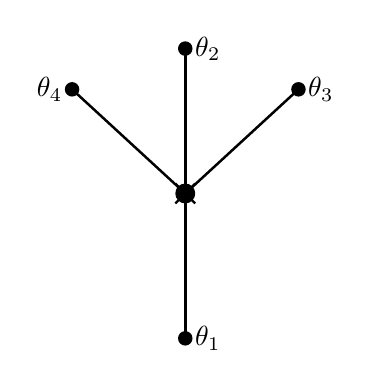
\begin{tikzpicture}[scale=1.15]
    \coordinate (O) at (0,0);

    \draw[line width=0.9pt] (O) -- (0,-1.6);
    \draw[line width=0.9pt] (O) -- (0,1.6);
    \draw[line width=0.9pt] (O) -- (1.25,1.15);
    \draw[line width=0.9pt] (O) -- (-1.25,1.15);

    \fill (O) circle (0.11);
    \draw[line width=0.8pt] (-0.11,-0.11) -- (0.11,0.11);
    \draw[line width=0.8pt] (-0.11,0.11) -- (0.11,-0.11);

    \fill (0,-1.6) circle (0.08);
    \fill (0,1.6) circle (0.08);
    \fill (1.25,1.15) circle (0.08);
    \fill (-1.25,1.15) circle (0.08);

    \node[right] at (0,-1.6) {$\theta_1$};
    \node[right] at (0,1.6) {$\theta_2$};
    \node[right] at (1.25,1.15) {$\theta_3$};
    \node[left] at (-1.25,1.15) {$\theta_4$};
\end{tikzpicture}
\end{center}

\[
\frac{\partial^2 V_{\text{eff}}}{\partial \theta^2}
=
m\ell^2\omega_0^2\cos\theta
\left(
1+\frac{b^2}{2}\cos\theta
\right)
-
m\ell^2\omega_0^2\sin^2\theta
\left(
\frac{b^2}{2}
\right)
\]

\[
\left.
\frac{d^2 V_{\text{eff}}}{d\theta^2}
\right|_{\theta=0}
=
m\ell^2\omega_0^2
\left(
1+\frac{b^2}{2}
\right)
>
0
\]

Stabile sempre.

\[
\left.
\frac{d^2 V_{\text{eff}}}{d\theta^2}
\right|_{\theta=\pi}
=
-m\ell^2\omega_0^2
\left(
1-\frac{b^2}{2}
\right)
=
m\ell^2\omega_0^2
\left(
\frac{b^2}{2}-1
\right)
>
0
\Longleftrightarrow
b^2>2
\]

Stabile per $b^2>2$ (ovvero $b>\sqrt{2}$), che è esattamente la condizione di esistenza per $\theta_{3,4}$.
\[
\left.
\frac{d^2V_{\text{eff}}}{d\theta^2}
\right|_{\theta_3,\theta_4}
=
m\ell^2\omega_0^2
\left(
-\frac{2}{b^2}
\right)
\left(
1+\frac{b^2}{2}
\left(
-\frac{2}{b^2}
\right)
\right)
-
m\ell^2\omega_0^2
\frac{b^2}{2}
\left(
1-\frac{4}{b^4}
\right)
=
-m\ell^2\omega_0^2
\left(
\frac{b^2}{2}
-
\frac{2}{b^2}
\right)
<0
\]

Instabile per $b^2>2$, ovvero ogni volta che esistono $\theta_{3,4}$.

\begin{center}
\begin{tikzpicture}[scale=1.15,>=Latex]

    % -------------------- caso b^2 < 2 --------------------
    \begin{scope}[xshift=-3.9cm]
        \node at (-1.7,1.35) {$b^2<2$};

        % assi
        \draw[->,line width=0.8pt] (-1.6,0) -- (2.1,0);
        \draw[->,line width=0.8pt] (0,-1.25) -- (0,1.45);

        % origine e pi
        \fill (0,0) circle (0.04);
        \node[above right] at (0,0) {$0$};

        \draw[dashed,line width=0.8pt] (1.75,0) -- (1.75,1.05);
        \node[below] at (1.75,0) {$\pi$};

        % etichetta V
        \node at (1.95,1.05) {$V$};

        % curva del potenziale
        \draw[line width=1pt]
            plot[smooth,tension=0.75] coordinates {
                (-1.55,0.90)
                (-1.25,0.75)
                (-0.85,0.25)
                (-0.45,-0.72)
                (0.10,-0.95)
                (0.70,-0.65)
                (1.15,0.00)
                (1.45,0.55)
                (1.75,0.85)
            };
    \end{scope}

    % -------------------- caso b^2 > 2 --------------------
    \begin{scope}[xshift=3.4cm]
        \node at (2.0,0.25) {$b^2>2$};

        % assi
        \draw[->,line width=0.8pt] (-1.4,0) -- (2.4,0);
        \draw[->,line width=0.8pt] (0,-1.25) -- (0,1.45);

        % origine
        \fill (0,0) circle (0.04);
        \node[below left] at (0,0) {$0$};

        % tacche sull'asse
        \draw[line width=0.8pt] (0.90,0.07) -- (0.90,-0.07);
        \node[below] at (0.90,0) {$\theta_3$};

        \draw[line width=0.8pt] (1.35,0.07) -- (1.35,-0.07);
        \node[below] at (1.35,0) {$\pi$};

        \draw[line width=0.8pt] (1.80,0.07) -- (1.80,-0.07);
        \node[below] at (1.80,0) {$\theta_4$};

        % etichetta V
        \node[red] at (1.75,1.05) {$V$};

        % curva del potenziale
        \draw[red,line width=1pt]
            plot[smooth,tension=0.9] coordinates {
                (-0.65,-1.00)
                (-0.25,-0.95)
                (0.15,-0.70)
                (0.50,0.10)
                (0.85,0.85)
                (1.15,0.70)
                (1.35,0.55)
                (1.60,0.72)
                (1.85,0.90)
                (2.10,0.45)
                (2.20,0.05)
            };
    \end{scope}

\end{tikzpicture}
\end{center}
